%        File: memoria.tex
%     Created: sáb jun 28 01:00  2008 C
% Last Change: sáb jun 28 01:00  2008 C
%
\documentclass[a4paper,spanish,12pt]{book}
\title{BLAS: Base Layer for Application Services}
\author{Eduardo Orive Vinuesa}
\usepackage{babel}
\usepackage{times}
\usepackage[T1]{fontenc}
\usepackage[utf8]{inputenc}
\usepackage[left=2.5cm, right=2.5cm]{geometry}
\usepackage{a4}
\usepackage{makeidx}
\usepackage{graphicx}
\usepackage{float}
\usepackage{url}
\usepackage{setspace}
\onehalfspacing
\usepackage{fancyheadings}

\begin{document}
\tableofcontents

\maketitle

%cuerpo del documento


\chapter*{Introducción}
Actualmente casi la totalidad de las instalaciones inform\'aticas son redes, y una mayoria de estas est\'an conectadas a Internet o incluso la propia Internet forma parte de estas. 

Es en este entorno donde se desarrollan las arquitecturas de la mayor\'ia de los sistemas. Distribuidas y en una gran proporci\'on siguiendo el modelo Cliente-Servidor casi todas las nuevas aplicaciones o sistemas basan gran parte de su funcionalidad en la conectividad mediante redes. 

Sin embargo realizar aunque sea un prototipo de un servicio de red resulta caro en tiempo y no se obtienen resultados tangibles hasta que se han implementado una buena parte del codigo.
Tambi\'en muy com\'un ver que muchos prototipos sean descartados (total o parcialmente) y deban re-escribirse ya que, aunque su rendimiento sea aceptable, la seguridad que ofrecen no lo es, con lo que el proceso de crear el servicio duplica su coste cuando el sistema llega a la etapa de producci\'on.

No obstante la escritura de un servicio de Red puede reducirse considerablemente si se implementan tan solo las caracteristicas particulares de su protocolo. Basicamente cualquier protocolo puede entenderse como un automata m\'as o menos complejo, siguiendo este modo de dise\~{o} puede simplificarse de manera considerable el trabajo del programador.
Existen multitud de funcionalidades ligadas a los programas que ofrecen servicios TCP que consumen mucho tiempo y que normalmente su implementaci\'on resulta bastante repetitiva:
\begin{enumerate}
	\item Entrada controlada de datos.
	\item Registro (o registros) de actividad y error.
	\item Lectura de los archivos de configuraci\'on.
	\item Parseado de los parametros de arraque.
\end{enumerate}

\chapter{Motivación}
Esta plataforma se ha pensado para los colectivos que por diversos motivos se ven ante la necesidad de programar un servicio de red en poco tiempo. A continuaci\'on se presentan varios de los perfiles de proyectos que se han planteado:
\section{Tipos de proyectos}
\subsection{Docencia}
Existen numerosos proyectos academicos que requieren la implementaci\'on de:
\begin{enumerate}
	\item Protocolos nuevos,
	\item Protocolos ya existentes.
	\item Modificaciones sobre protocolos antiguos. 
\end{enumerate}

\subsection{Microdispositivos}
La mayor\'ia de los dispositivos dotados de un sistema operativo m\'inimo disponen de una modesta pila TCP/IP ya que practicamente todos estos dispositivos se dise\~{n}an incluyendo algún tipo de hardware de interconexi\'on. Sin embargo por razones de coste economico o rendimiento energetico siguen afectados por una leve capacidad de memoria y/o potencia de c\'alculo que hacen que la opcion de conectarlos a un servicio convencional (HTTP y REST por ejemplo) resulte muy engorrosa (y caro) en su programaci\'on, e incluso a veces impracticable.

Es por este motivo que se suelen dise\~{n}ar protocolos normalmente muy escuetos, especificamente adaptados a la funcionalidad del dispositivo y a sus limitaciones de proceso.

\subsection{Seguridad Inform\'atica}
En un entorno en que los ataques mediante gusanos son casi rutinarios se emplea mucho tiempo y esfuerzo en crear servicios que se comporten como los originales que emplee el gusano para penetrar en el sistema y as\'i poder estudiar que acciones realiza una vez dentro.

La capacidad de programar servicios simulados agilmente puede ser un complemento perfecto a otras herramientas de estudio de la seguridad como son las 'Honey-Nets', dotando a las m\'aquinas virtuales de un comportamiento mucho m\'as flexible.

\subsection{Elecci\'on del Lenguaje} 
Se ha elegido Python como lenguaje de programaci\'on para esta plataforma por las siguientes razones:
\begin{enumerate}
	\item Velocidad de aprendizaje: cualquier persona que conozca un lenguaje orientado a objetos puede aprenderlo en muy poco tiempo.
	\item Reflexividad: Las clases en pytohn tienen conocimiento de sus propios metodos y atributos.
	\item Interpretado: Al ejecutarse bajo un interprete no har\'an falta compilar distintos ejecutables seg\'un la plataforma.
\end{enumerate}

Con el empleo de Python se puede conseguir con pocas lineas la implementaci\'on de un protocolo completo. Al tratarse de un lenguaje en que la identaci\'on es obligatoria y la sintaxis muy clara normalmente su codigo fuente esta bien estructurado y resulta facil de leer incluso para quienes apenas conozcan Python.

\chapter{protocolos}
En este proyecto se van a implementar una serie de protocolos para demostrar la versatilidad de la plataforma y sobre todo la comodidad y la limpieza de codigo que aportan. Los protocolos elegidos son los siguientes
\section{Telnet}
Se trata de un cl\'asico obligatorio entre cualquier servicio de red. Se trata de un protocolo que permite el control de una terminal 
\section{HTTP: HiperText Transfer Protocol}
Elaborado por el W3C y la IETF el HTTP es seguramente uno de los servicios de red más extendido en internet y en redes internas. Define las normas de comunicación entre los participantes del servicio (clientes, servidores y opcionalmente proxies). Servirá como ejemplo para abordar la programacion de un protocolo m\'as avanzado y permita su uso desde los diversos tipos de navegadores.
\section{SIP: Session Initiation Protocol} 
Es un protocolo desarrollado por el IETF MMUSIC Working Group en la busqueda de un estandar para iniciar, finalizar o modificar sesiones interactivas de usuario, que se emplearan para contactar con dichos usuarios. Normalmente se utiliza en conjunción con otros servicios, principalmente multimedia (video, voz, mensajeria instantanea). Se ha convertido en el protocolo de señalización para voz por IP más utilizado junto al H.232.

\chapter{Análisis}
El modelo Cliente-Servidor es tan básico de entender como antiguo, se pueden considerar que los primeros sistemas de este tipo eran los teletipos utilizados en las universidades para emitir programas a los equipos que alli habian instalados y recibir posteriormente sus resultados. A diferencia de hoy aquellos sistemas funcionaban directamente sobre enlaces dedicados y cada uno de estos teletipos disponia de una conexión permanente.

Sin embargo la implantación de sistemas de red por capas, enlaces no dedicados y sobre todo la diversificación de equipos mucho mas baratos y potentes han modificado el panorama de manera importante: Además de diversificarse los tipos de servicios era posible que varios de ellos coexisitieran en el mismo equipo.


\begin{figure}
	  \centering
	      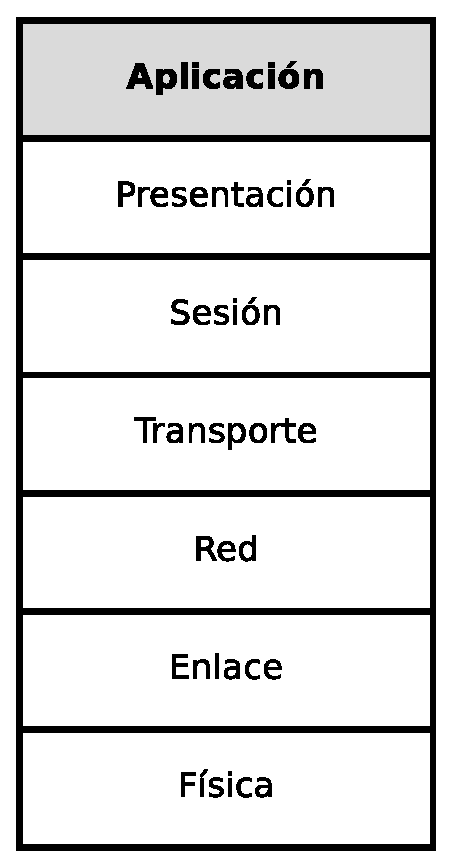
\includegraphics{img/NivelesOSI.mp}
              \caption{niveles OSI}
  \label{fig:ejemplo}
\end{figure}

[niveles OSI]

Limitando la comunicación al nivel de aplicación todos los protocolos existentes pueden resumirse como una secuencia de emisión y recepción de datos en una serie de etapas y formatos establecidos por el protocolo. 
De esta manera se puede entender al servicio como un autómata sensible al contexto para cada conexión que recibe. Orientando el diseño del servicio como una secuencia de pasos y que estos sean lo más simple y claro posible se ahorrará mucho tiempo y complejidad en la producción del codigo. 

Además de la programación del propio protocolo se deben implementar ciertas funciones como son:
\begin{enumerate}
	\item La lectura de parámetros desde linea de comandos
	\item La lectura de parámetros desde el archivo de configuracion
	\item El registro de actividad en el(los archivo(s) pertinentes
	\item Distintos modos de entrada de datos
\end{enumerate}


\end{document}

